\documentclass[14pt]{extreport}
\usepackage{gost}
\usepackage{lscape}
\usepackage{multirow}





\begin{document}
\begin{figure}[]
		
\includegraphics[scale=0.66]{itmo_image.png}
		\label{pic1}
\end{figure}
\begin{flushleft}
\begin{tabular}{ p{9cm}p{8cm} }
 Группа: K3120 & К работе допущен: \\ 
 Студент: Скворцов И.В. & Работа выполнена: \\  
 Преподаватель: Попов А. С. & Отчет принят: \\    
\end{tabular}
\end{flushleft}

\begin{center}
\Large\textbf{Рабочий протокол и отчёт по\\лабораторной работе №1.01}

\large\textbf{Исследование распределения случайной величины}
\end{center}

\section*{1. Цель работы.}

\begin{enumerate}
    \item Провести многократные измерения определенного интервала времени. 
    \item Проверить зависимость момента инерции от положения масс относительно оси вращения.
\end{enumerate}


\section*{2. Задачи.}
\begin{enumerate}
    \item Провести многократные измерения временного интервала, размером 7 секунд.
    \item Построить гистограмму распределения результатов измерений.
    \item Вычислить среднее значение и дисперсию полученной выборки.
    \item Сравнить гистограмму с графиком функции Гаусса с аналогичным экспериментальному распределением, средним значением и дисперсией.
\end{enumerate}

\section*{3. Объект исследования.}
Распределение случайной величины.

\section*{4. Метод экспериментального исследования.}
Используя стрелочный секундомер, устанавливается интервал в 7 секунд, который затем измеряется неоднократно с помощью цифрового секундомера.

\section*{5. Рабочие формулы и исходные данные.}
Выборочное среднее как среднее арифметическое всех результатов измерений:
\begin{equation}\label{f1}
    \langle t \rangle_N = \frac{1}{N}(t_1+t_2+\dotsb+t_N)=\frac{1}{N}\displaystyle\sum_{i=1}^{N} t_i
\end{equation}

Выборочное среднеквадратичное отклонение:
\begin{equation}\label{f3}
    \sigma_N = \sqrt{\frac{1}{N-1}\displaystyle\sum_{i=1}^{N} (t_i - \langle t \rangle_N)^2}
\end{equation}

Значение плотности вероятности:
\begin{equation}\label{f2}
    \rho(t) = \frac{\Delta N}{N \Delta t}
\end{equation}

Максимальное значение плотности распределения:
\begin{equation}\label{f4}
    \rho_{max} = \frac{1}{\sigma\sqrt{2\pi}}
\end{equation}

Функция Гаусса:
\begin{equation}\label{f5}
    \rho(t) = \frac{1}{\sigma\sqrt{2\pi}}\exp{\left(-\frac{(t - \langle t \rangle_N)^2}{2\sigma^2}\right)}
\end{equation}
\newpage

Значения вероятности попадания результата каждого измерения $t$ в интервал $[t_1; t_2]$ в стандартных(наиболее употребительных на практике) интервалах при условии реализации нормального распределения случайной величины:


\begin{equation*}\label{f6}
    t \in [\langle t \rangle_N - \sigma, \langle t \rangle_N + \sigma], P_{\sigma} \cong 0,683
\end{equation*}
\begin{equation}\label{f7}
    t \in [\langle t \rangle_N - 2\sigma, \langle t \rangle_N + 2\sigma], P_{2\sigma} \cong 0,954
\end{equation}
\begin{equation*}\label{f8}
    t \in [\langle t \rangle_N - 3\sigma, \langle t \rangle_N + 3\sigma], P_{3\sigma} \cong 0,997
\end{equation*}

Формулы для вычисления приближённой вероятности попадания каждого измерения $t$ в интервал $[t_1; t_2]$:
\begin{equation*}\label{f9}
    t \in [\langle t \rangle_N - \sigma_N, \langle t \rangle_N + \sigma_N]
\end{equation*}
\begin{equation}\label{f10}
    t \in [\langle t \rangle_N - 2\sigma_N, \langle t \rangle_N + 2\sigma_N]
\end{equation}
\begin{equation*}\label{f11}
    t \in [\langle t \rangle_N - 3\sigma_N, \langle t \rangle_N + 3\sigma_N]
\end{equation*}

Доверительный интервал для промежутка времени, который измеряется в ходе работы:
\begin{equation}\label{f12}
    \Delta t = t_{\alpha, N} \cdot \sigma_{\langle t \rangle}
\end{equation}

\section*{6. Измерительные приборы.}
\begin{table}[H]\label{t1}
\caption{Измерительны приборы.}
\centering
\begin{tabular}{|c|c|c|c|c|}
\hline
 № и/п & Наименование & Тип прибора & Используемый & Погрешность \\ 
 & & & диапазон, с & прибора, с \\ \hline
 1 & Секундомер стрелочный & Стрелочный & [0; 60] & 0.01 \\ \hline
 2 & Секундомер цифровой & Цифровой & [0; 60] & 0.0005 \\ \hline
 
\end{tabular}
\end{table}

\section*{7. Результаты прямых измерений.}
\begin{table}[H]\label{t2}
\caption{Результаты прямых измерений и их обработки .}
\small
\centering
\begin{tabular}{|c|c|c|c|c|c|c|c|}
\hline
 № & $t_i$, c & $t_i - \langle t \rangle_N$, c & $(t_i - \langle t \rangle_N)^2$, $\mathrm{c}^2$ & № & $t_i$, c & $t_i - \langle t \rangle_N$, c & $(t_i - \langle t \rangle_N)^2$, $\mathrm{c}^2$ \\
 \hline
        1 & 6,71 & -0,23904 & 0,057140122  & 26 & 6,764 & -0,18504 & 0,034239802  \\ \hline
        2 & 6,867 & -0,08204 & 0,006730562  & 27 & 6,965 & 0,01596 & 0,000254722  \\ \hline
        3 & 7,15 & 0,20096 & 0,040384922  & 28 & 7,165 & 0,21596 & 0,046638722  \\ \hline
        4 & 6,907 & -0,04204 & 0,001767362  & 29 & 6,866 & -0,08304 & 0,006895642  \\ \hline
        5 & 6,962 & 0,01296 & 0,000167962  & 30 & 6,815 & -0,13404 & 0,017966722  \\ \hline
        6 & 6,837 & -0,11204 & 0,012552962  & 31 & 6,966 & 0,01696 & 0,000287642  \\ \hline
        7 & 7,27 & 0,32096 & 0,103015322  & 32 & 7,017 & 0,06796 & 0,004618562  \\ \hline
        8 & 6,966 & 0,01696 & 0,000287642  & 33 & 6,863 & -0,08604 & 0,007402882  \\ \hline
        9 & 7,167 & 0,21796 & 0,047506562  & 34 & 6,866 & -0,08304 & 0,006895642  \\ \hline
        10 & 7,424 & 0,47496 & 0,225587002  & 35 & 6,559 & -0,39004 & 0,152131202  \\ \hline
        11 & 7,427 & 0,47796 & 0,228445762  & 36 & 7,171 & 0,22196 & 0,049266242  \\ \hline
        12 & 6,865 & -0,08404 & 0,007062722  & 37 & 6,816 & -0,13304 & 0,017699642  \\ \hline
        13 & 7,015 & 0,06596 & 0,004350722  & 38 & 6,663 & -0,28604 & 0,081818882  \\ \hline
        14 & 6,403 & -0,54604 & 0,298159682  & 39 & 6,966 & 0,01696 & 0,000287642  \\ \hline
        15 & 7,018 & 0,06896 & 0,004755482  & 40 & 7,018 & 0,06896 & 0,004755482  \\ \hline
        16 & 6,81 & -0,13904 & 0,019332122  & 41 & 6,814 & -0,13504 & 0,018235802  \\ \hline
        17 & 6,986 & 0,03696 & 0,001366042  & 42 & 7,013 & 0,06396 & 0,004090882  \\ \hline
        18 & 7,119 & 0,16996 & 0,028886402  & 43 & 6,967 & 0,01796 & 0,000322562  \\ \hline
        19 & 6,967 & 0,01796 & 0,000322562  & 44 & 7,017 & 0,06796 & 0,004618562  \\ \hline
        20 & 7,125 & 0,17596 & 0,030961922  & 45 & 6,815 & -0,13404 & 0,017966722  \\ \hline
        21 & 6,664 & -0,28504 & 0,081247802  & 46 & 7,021 & 0,07196 & 0,005178242  \\ \hline
        22 & 6,866 & -0,08304 & 0,006895642  & 47 & 6,972 & 0,02296 & 0,000527162  \\ \hline
        23 & 7,245 & 0,29596 & 0,087592322  & 48 & 7,121 & 0,17196 & 0,029570242  \\ \hline
        24 & 6,814 & -0,13504 & 0,018235802  & 49 & 6,813 & -0,13604 & 0,018506882  \\ \hline
        25 & 6,819 & -0,13004 & 0,016910402 & 50 & 7,016 & 0,06696 & 0,004483642 \\ \hline
        & \multicolumn{1}{c|}{$\langle t \rangle_N = 6.949, c$}& \multicolumn{3}{c|}{$\sum\limits_{i=1}^N(t_i - \langle t \rangle) = -6,21725 * 10^{-15}, c$}& \multicolumn{2}{c|}{ $\sigma_N = 0.19506, c$} & $\rho_{max} =   2,04523, c^{-1}$ \\ 
        \hline 
\end{tabular}
\normalsize
\end{table}

\section*{8. Расчёт результатов косвенных измерений.}

Среднее арифметическое значение результатов измерений:
\begin{equation*}
    \langle t \rangle_N = \frac{347,452}{50} = 6,949 \text{, c}
\end{equation*}

Выборочное среднеквадратичное отклонение:
\begin{equation*}
    \sigma_N = \sqrt{\frac{1,86432592}{49}} = 0.19506 \text{, с}
\end{equation*}

Максимальное значение плотности распределения:
\begin{equation*}
    \rho_{max} = \frac{1}{0.19506 \cdot 2,50663} = 2,04523 \text{, с}^{-1}
\end{equation*}

Среднеквадратичное отклонение среднего значения:
\begin{equation*}
    \sigma_{\langle t \rangle} = \sqrt{\frac{1,86432592}{2450}} = 0,0275853 \text{, с}
\end{equation*}

\begin{table}[H]
\caption{Стандартные доверительные интервалы.}
\centering
\begin{tabular}{|c|c|c|c|c|c|c|}
\hline
& Начало интервала, с & Конец интервала, с &  $\Delta N$ & $\frac{\Delta N}{N}$ & $P$ \\ \hline
$\langle t \rangle_N \pm \sigma_N$ & 6,754 & 7,144 & 37 & 0,74 & 0,683\\ \hline
$\langle t \rangle_N \pm 2\sigma_N$ & 6,559 & 7,340 & 47 & 0,94 & 0,954 \\ \hline
$\langle t \rangle_N \pm 3\sigma_N$ & 6,364 & 7,534 & 50 & 1,00 &  0,997 \\ \hline
 \end{tabular}
\end{table}

Среди полученных данных $t_{min} = 6,403$ и $t_{max} = 7,427$ Разобьем промежуток [6,403; 7,427] на $\sqrt{N} \approx 7$ равных частей: $\Delta t =  0,15$.
\begin{table}[H]
\caption{Данные для построения гистограммы.}

\centering
\begin{tabular}{|c|c|c|c|c|}
\hline
Интервал & $\Delta N$ & $\frac{\Delta N}{N \Delta t}, \text{ с}^{-1}$ & $t, \text{с}$ & $\rho, \text{ с}^{-1}$ \\ \hline
[6,40; 6,55] & 1 & 0,13 & 6,475 & 0,1067259319626144 \\ \hline
[6,55 ; 6,70] & 3 & 0,4 & 6,625 & 0,5146145682042214 \\ \hline
[6,70; 6,85] &  11 & 1,47 & 6,775 & 1,373641115817862 \\ \hline
[6,85; 7,00] & 16 & 2,13 & 6,925 & 2,0297547733335524 \\ \hline
[7,00; 7,15] & 11 & 1.47 & 7,075 & 1,6603243825081777 \\ \hline
[7,15; 7,30] & 6 & 0,8 & 7,225 & 0,7518330354561166 \\ \hline
[7,30; 7,45] & 2 & 0,27 & 7,375 & 0,18846423594138365 \\ \hline

 \end{tabular}
\end{table}

\section*{9. Расчёт погрешности измерений.}

Коэффицент Стьюдента для доверительной вероятности $\alpha = 0,95$: $$t_{\alpha, N} = 2.0086$$

Доверительный интервал:

$$\Delta t = t_{\alpha, N} \cdot \sigma_{\langle t \rangle} = 0,0575429358 \approx 0,06 \text{ с}$$

\section*{10. Графики(перечень графиков, которые составляют Приложение 1)}
\begin{figure}[H]
	\begin{center}
		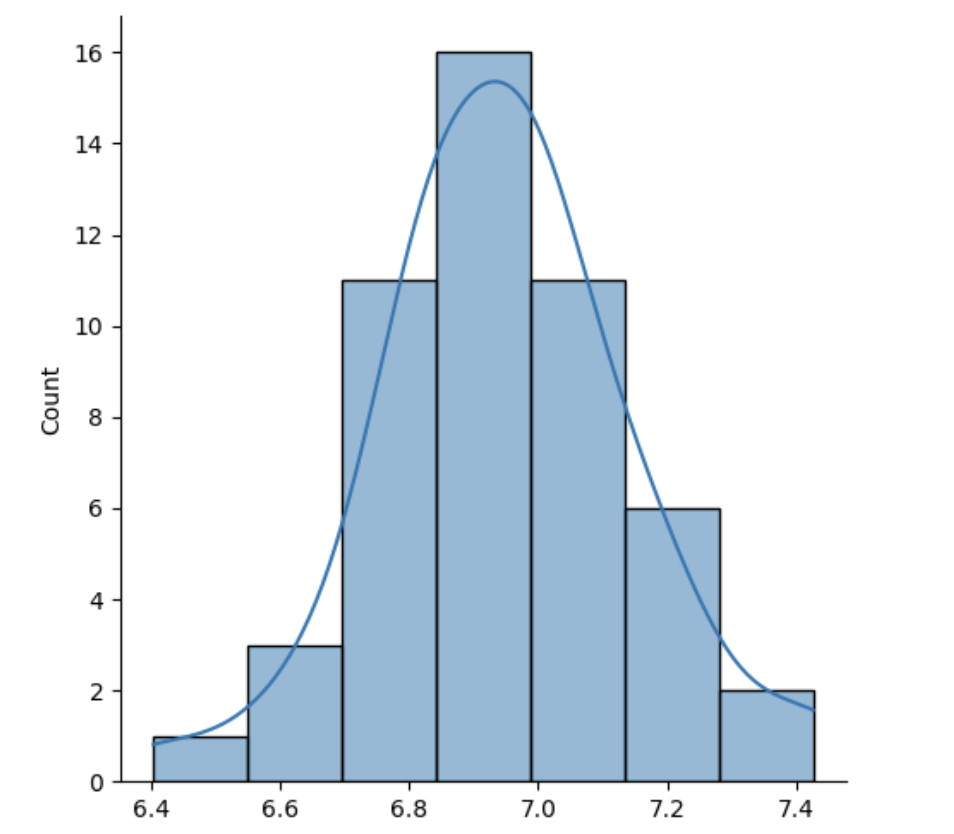
\includegraphics[scale=1]{dristogramma.png}
		\caption{Распределение результатов измерения}
		\label{pic}
	\end{center}
\end{figure}

\section*{11. Окончательные результаты.}
Доверительный интервал:
\begin{equation*}
    t = 6,95 \pm 0,06 \text{ с при } \alpha = 0,95
\end{equation*}

Относительная погрешность измерений:
\begin{equation*}
    \varepsilon = \frac{\Delta t}{\langle t \rangle_N} \cdot 100\% = 0,008280750582818 \cdot 100\% \approx 0,83\%
\end{equation*}

\section*{12. Выводы и анализ результатов работы.}
В ходе лабораторной работы мы исследовали закон распределения случайной величины на примере многократных измерений заранее определенного интервала времени. Для этих данных был вычислен доверительный интервал, среднее квадратичное отклонение, максимальное значение плотности распределения и среднеквадратичное отклонение среднего значения. На основании полученных данных была построена гистограмма и график функции распределения плотности. График показал, что исследуемое распределение соответствет нормальному.
\end{document}
